This region is defined to select $\zmumuplusjets$ processes and is used in the
estimation of the V + jets background contribution in the signal region. It is
defined in the same way as in
\cref{sec:di-muon-control}. \cref{fig:dimu_cr_plots} reports the $\met$ and
leading jet $\pt$ distributions, it can be seen that there is a good agreement
between data and \gls{mc} prediction within uncertainties.
\begin{figure}[!th]
  \centering
  \begin{subfigure}[t]{.48\linewidth}
    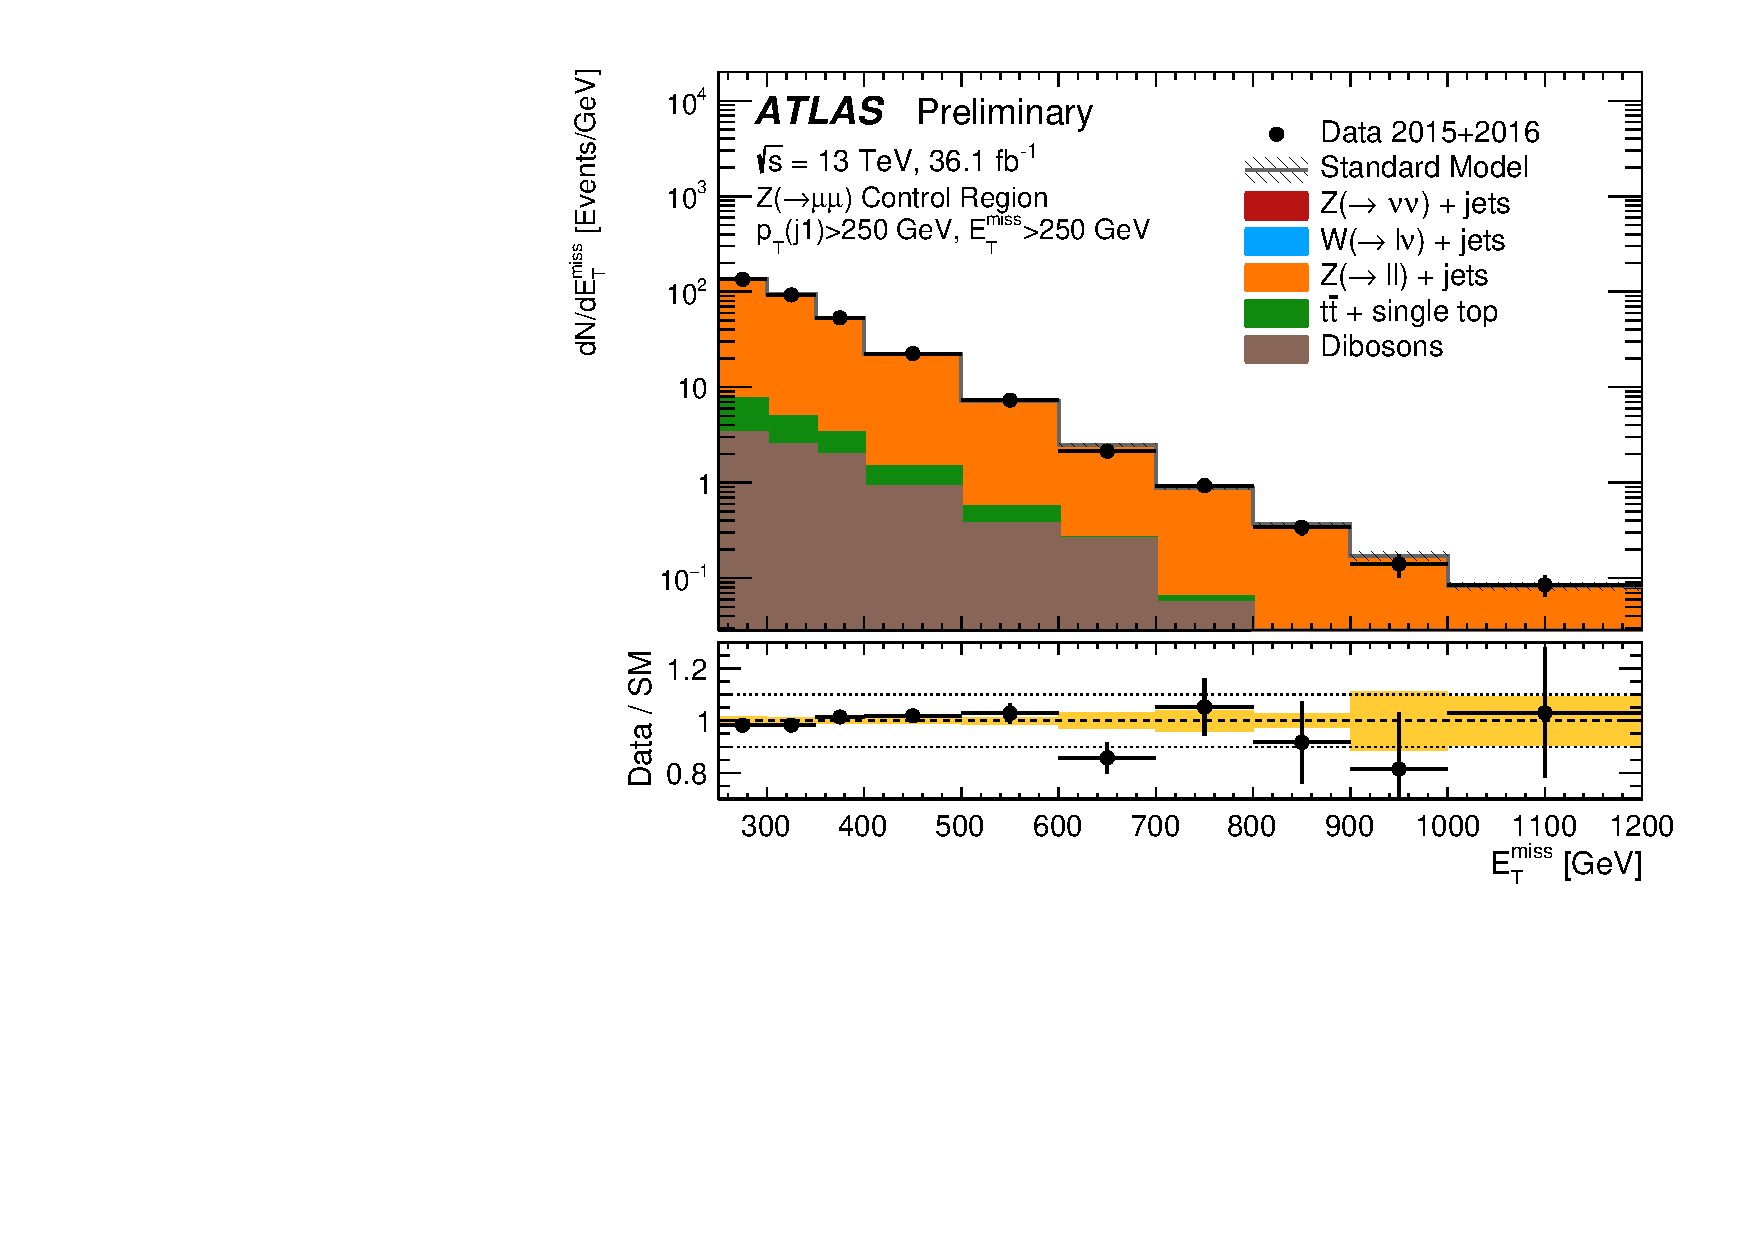
\includegraphics[width=\linewidth]{zmumu_cr_met}
    \caption{$\met$ distribution.}
    \label{fig:dimu_cr_met}
  \end{subfigure}
  \begin{subfigure}[t]{.48\linewidth}
    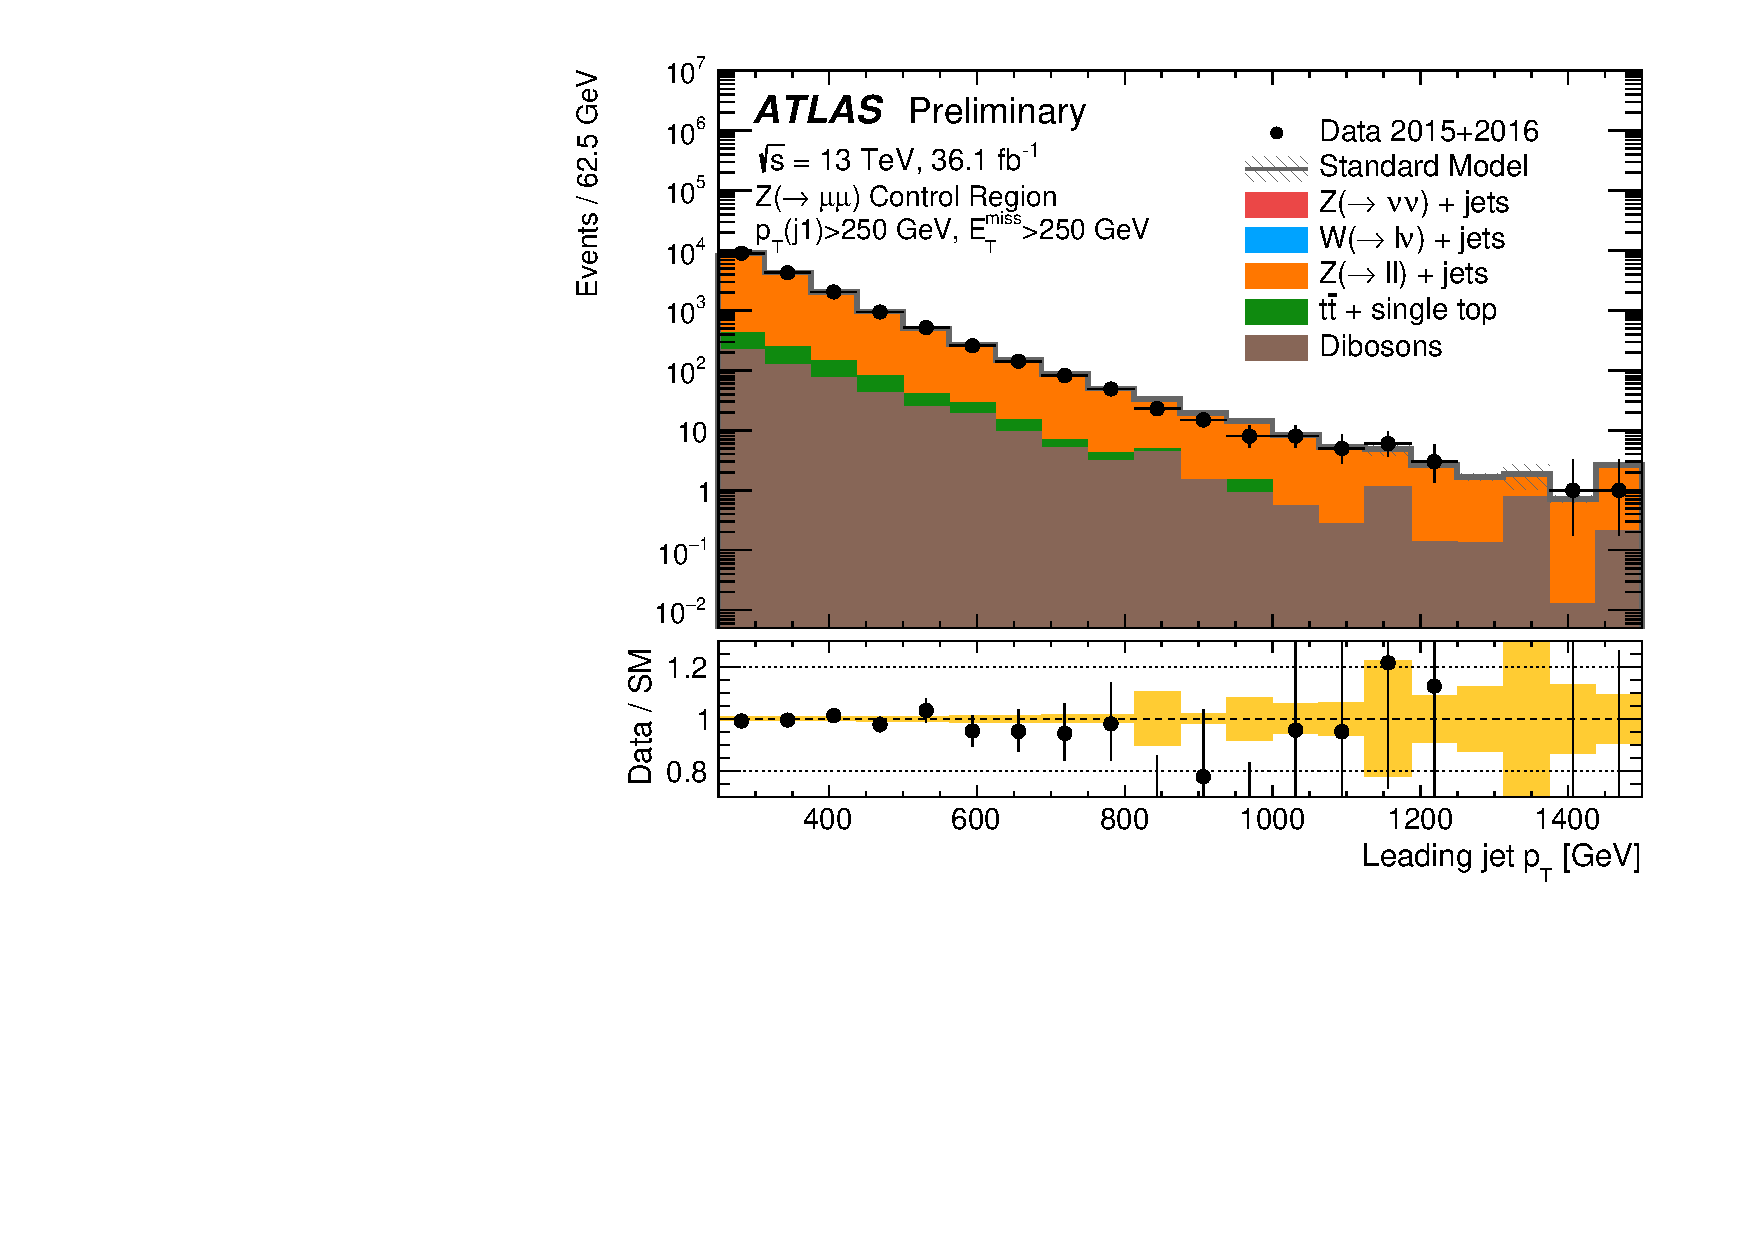
\includegraphics[width=\linewidth]{zmumu_cr_jet1}
    \caption{Leading jet $\pt$ distribution.}
    \label{fig:dimu_cr_jet1}
  \end{subfigure}
  \caption{Observed and predicted $\met$ and leading jet $\pt$ after the
    background only fit in the $\crzmm$ control region for the $\met > 250$~GeV
    inclusive selection corresponding to IM1. The error bands in the ratio plot
    on the bottom of the figures include statistical and systematic
    uncertainties. The negligible contribution of \gls{ncb} and diboson
    backgrounds is not reported in the figure.}
  \label{fig:dimu_cr_plots}
\end{figure}
%%% Local Variables:
%%% mode: latex
%%% TeX-master: "../search_for_DM_LED_with_ATLAS"
%%% End:
